%
%	Begrifflichkeiten
%

\pagebreak
\section{Data Sources and Research Methods}

\onehalfspacing

\subsection{Original Data}

For this paper's data analysis and visualization, we will use raw benchmark data from the original author's Github pages for the years \href{https://github.com/InfraBuilder/benchmark-k8s-cni-2024-01}{2024}, \href{https://github.com/InfraBuilder/benchmark-k8s-cni-2021-05}{2021}, and \href{https://github.com/InfraBuilder/benchmark-k8s-cni-2020-08}{2020} and perform a secondary data analysis.\footnote{See \textit{Jillier, W. (2021)}: A Guide To Secondary Data Analysis. \cite{secondaryDA}} We will use the previously collected measurements instead of gathering new data to answer our research question.

In their 2024 article, Alexis Ducastel recommended Cilium as the preferred CNI for RKE2.

\subsection{Data Wrangling}

To support the secondary analysis, we had to convert the original raw data into a common format. The CSV format is widely supported in statistical analysis, so we chose this as the target format.

\subsubsection{2020 and 2021 - adding Header information}

The original raw data for 2020 and 2021 are in tab-separated files without headers, split by CNI; they do not contain header information.

From the overall aggregated result spreadsheets, we added the following headers to the TSV Files and subsequently converted them to CSV format:

\begin{itemize}
    \item smem - "Server Memory (MB)"
    \item scpu - "Server CPU (\%)"
    \item cmem - "Client Memory (MB)"
    \item ccpu - "Client CPU (\%)"
    \item tcpbw - "TCP Pod to Pod Bandwidth (Mbit/s)"
    \item tcpsm - "Server Memory (MB)"
    \item tcpsc - "Server CPU (\%)"
    \item tcpcm - "Client Memory (MB)"
    \item tcpcc - "Client CPU (\%)"
    \item udpbw - "UDP Pod to Pod Bandwidth (Mbit/s)"
    \item udpsm - "Server Memory (MB)"
    \item udpsc - "Server CPU (\%)"
    \item udpcm - "Client Memory (MB)"
    \item udpcc - "Client CPU (\%)"
    \item tcpebw - "TCP Pod to Service Bandwidth (Mbit/s)"
    \item tcpesm - "Server Memory (MB)"
    \item tcpesc - "Server CPU (\%)"
    \item tcpecm - "Client Memory (MB)"
    \item tcpecc - "Client CPU (\%)"
    \item udpebw - "UDP Pod to Service Bandwidth (Mbit/s)"
    \item udpesm - "Server Memory (MB)"
    \item udpesc - "Server CPU (\%)"
    \item udpecm - "Client Memory (MB)"
    \item udpecc - "Client CPU (\%)"
\end{itemize}

We also removed the discovered MTU size from the measurements, as it was a constant value and was not present in the 2024 data.

\subsubsection{2024 - Data Transformation}

The original raw data for 2024 is formatted as \href{https://prometheus.io/docs/concepts/metric_types/#gauge}{Prometheus gauges}, also split by CNI.

\begin{figure}[H]
\centering
\caption {2024 Flannel Results}
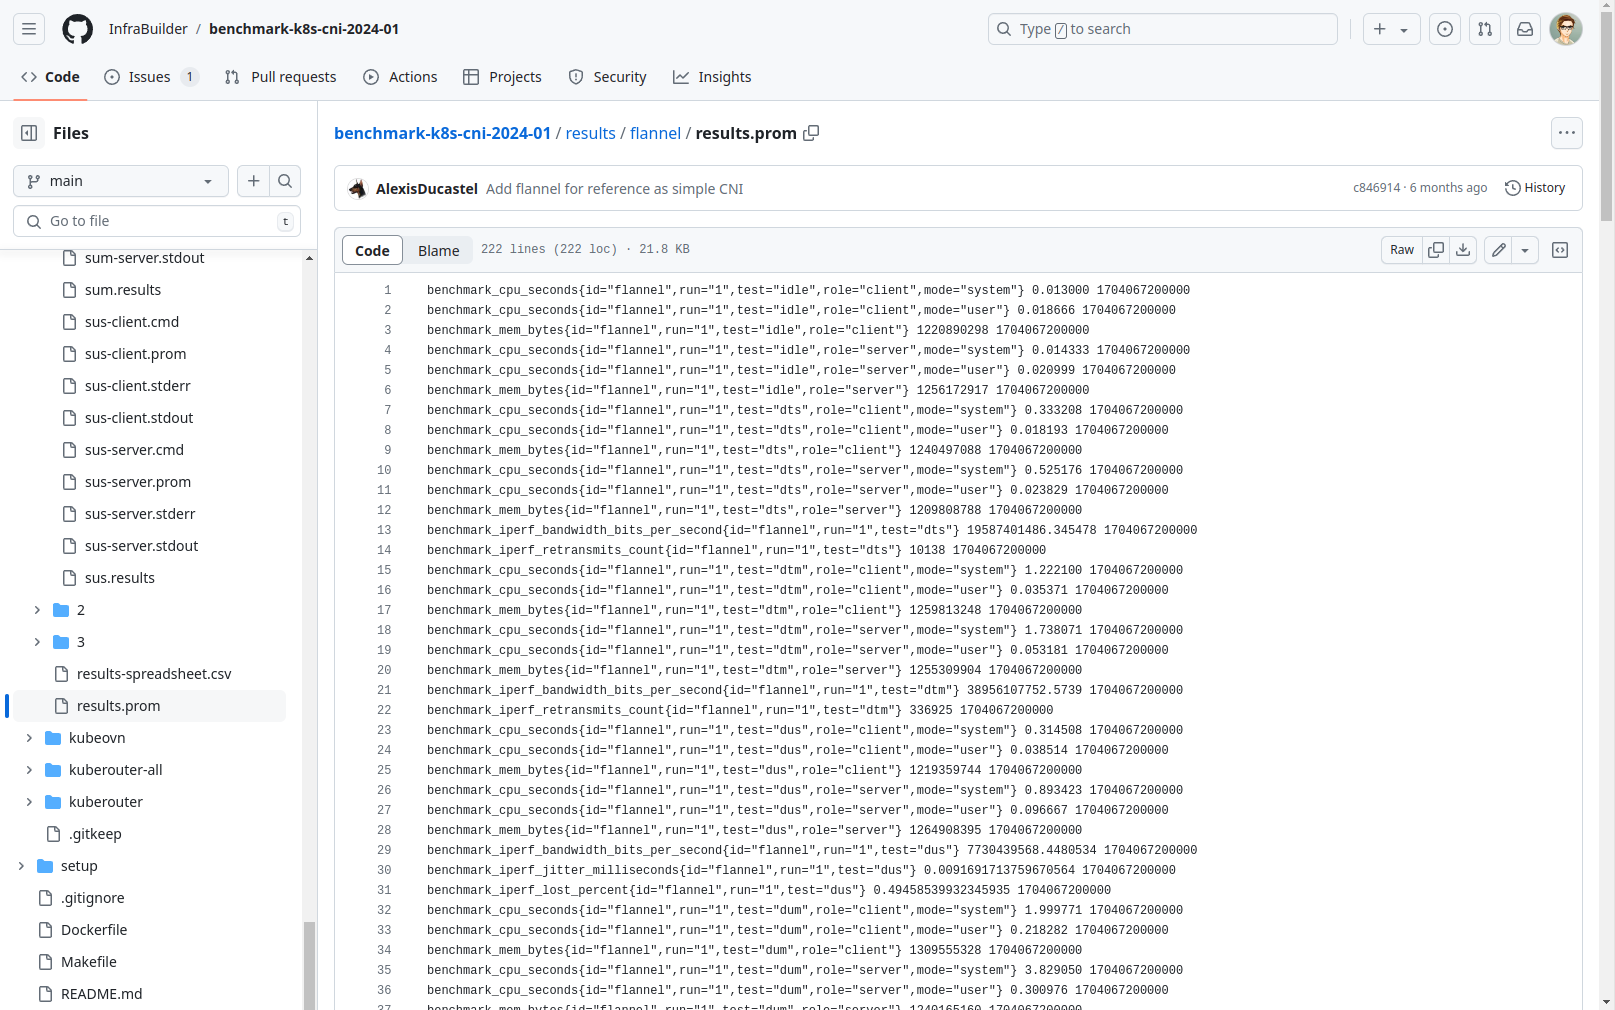
\includegraphics[width=\linewidth]{images/flannel-prom.png}
\label{fig:flannel-prom}
\end{figure}

As the 2024 data format was vastly different, we decided to convert the Prometheus gauges for easier handling. The 2024 data also had many more data points, so we mapped the gauges to the most appropriate fields and adjusted the scale where necessary (e.g., Bytes to Megabytes).

\begin{itemize}
    \item smem - "benchmark\_mem\_bytes - server - idle"
    \item scpu - "benchmark\_cpu\_seconds - server - idle"
    \item cmem - "benchmark\_mem\_bytes - client - idle"
    \item ccpu - "benchmark\_cpu\_seconds - client - idle"
    \item tcpbw - "benchmark\_iperf\_bandwidth\_bits\_per\_second - dts"
    \item tcpsm - "benchmark\_mem\_bytes - server - dts"
    \item tcpsc - "benchmark\_cpu\_seconds - server - dts"
    \item tcpcm - "benchmark\_mem\_bytes - client - dts"
    \item tcpcc - "benchmark\_cpu\_seconds - client - dts"
    \item udpbw - "benchmark\_iperf\_bandwidth\_bits\_per\_second - dus"
    \item udpsm - "benchmark\_mem\_bytes - server - dus"
    \item udpsc - "benchmark\_cpu\_seconds - server - dus"
    \item udpcm - "benchmark\_mem\_bytes - client - dus"
    \item udpcc - "benchmark\_mem\_bytes - client - dus"
    \item tcpebw - "benchmark\_iperf\_bandwidth\_bits\_per\_second - sts"
    \item tcpesm - "benchmark\_mem\_bytes - server - sts"
    \item tcpesc - "benchmark\_cpu\_seconds - server - sts"
    \item tcpecm - "benchmark\_mem\_bytes - client - sts"
    \item tcpecc - "benchmark\_cpu\_seconds - client - sts"
    \item udpebw - "benchmark\_iperf\_bandwidth\_bits\_per\_second - sus"
    \item udpesm - "benchmark\_mem\_bytes - server - sus"
    \item udpesc - "benchmark\_cpu\_seconds - server - sus"
    \item udpecm - "benchmark\_mem\_bytes - client - sus"
    \item udpecc - "benchmark\_mem\_bytes - client - sus"
\end{itemize}

\subsection{What's Not in the Data}

The benchmark data was originally recorded with the author's \href{https://github.com/InfraBuilder/k8s-bench-suite}{k8s-bench-suite}. Their test suite uses \href{https://iperf.fr/}{iPerf} for measurements and provides a convenient shell interface for data collection.

The data itself does not contain information on the infrastructure setup and the software versions used.

\begin{itemize}
    \item The \href{https://github.com/InfraBuilder/benchmark-k8s-cni-2020-08/blob/master/PROTOCOL.md}{2020 setup} was three \href{https://www.supermicro.com/en/}{Supermicro} bare-metal servers connected through a Supermicro 10Gbit switch, running \href{https://ubuntu.com/server}{Ubuntu} 18.04 LTS and Kubernetes 1.19.0.
\end{itemize}

\begin{table}[H]
\caption{2020 CNI Versions}
\begin{tabular}{|c | c | c | c |} 
 \hline
 Flannel & Calico & Canal & Cilium \\
 \hline
 v0.12.0 & v3.16.1 & v3.16.1 & v1.8.2 \\ 
 \hline
\end{tabular}
\label{tab:2020ver}
\end{table}

\begin{itemize}
    \item The \href{https://github.com/InfraBuilder/benchmark-k8s-cni-2021-05/blob/main/PROTOCOL.md}{2021 setup} was three Supermicro bare-metal servers connected through a Supermicro 10Gbit switch, running Ubuntu 20.04 LTS and Kubernetes 1.21.0.
\end{itemize}

\begin{table}[H]
\caption{2021 CNI Versions}
\begin{tabular}{|c | c | c | c |} 
 \hline
 Flannel & Calico & Canal & Cilium \\
 \hline
 v0.15.1 & v3.19.2 & v3.19.2 & v1.11.2 \\ 
 \hline
\end{tabular}
\label{tab:2021ver}
\end{table}

\begin{itemize}
    \item For 2024, the test infrastructure consisted of three Supermicro bare-metal servers connected through a Supermicro 40Gbit switch, running Ubuntu 22.04 LTS and Kubernetes 1.26.12.\footnote{See \textit{Ducastel, A. (2024)}: Benchmark results of Kubernetes network plugins. \cite{originalArticle}}
\end{itemize}

\begin{table}[H]
\caption{2024 CNI Versions}
\begin{tabular}{|c | c | c | c |} 
 \hline
 Flannel & Calico & Canal & Cilium \\
 \hline
 v0.24.3 & v3.27.2 & v3.27.2 & v1.15.2 \\ 
 \hline
\end{tabular}
\label{tab:2024ver}
\end{table}

\subsection{Data Exploration}

We will analyze the data sets using the methods of Exploratory Data Analysis (EDA).

John Tukey has promoted EDA since 1977 to encourage data scientists to explore data and formulate hypotheses that could lead to new data collection and experiments.\footnote{See \textit{Tukey, J.W. (1977)}: Exploratory data analysis. \cite{exploratoryDA}}

EDA uses statistical methods to analyze and visualize the data, understand key characteristics, and identify patterns and relationships. 

We will use summary statistics, such as mode, mean, and median, to understand the data and augment this with data visualization, e.g. histograms. We have already cleaned up the data and converted the data sets to a common format. EDA should help us to make informed decisions about how to proceed with our analysis and draw meaningful conclusions from the data. .\footnote{See \textit{Gemini (2024)}: Exploratory Data Analysis. \cite{bardExploratory}}  

We will not use the data to predict performance gains in future releases of the CNIs or through improved network speeds; instead, we will focus on our research question and attempt to arrive at a recommendation for CNI usage.

\subsection{Tools}

We performed most of the initial data wrangling with \href{https://www.gnu.org/software/bash/}{Bash} and \href{https://pubs.opengroup.org/onlinepubs/9699919799/utilities/vi.html}{vi}, and \href{https://www.microsoft.com/en-us/microsoft-365/excel}{Microsoft Excel} to support operations on columns.

For the subsequent data exploration, we will use \href{https://www.r-project.org/}{R} and \href{https://posit.co/download/rstudio-desktop/}{RStudio}.

\begin{Shaded}
\begin{Highlighting}[]
\NormalTok{version}
\end{Highlighting}
\end{Shaded}

\begin{verbatim}
platform       x86_64-w64-mingw32               
arch           x86_64                           
os             mingw32                          
crt            ucrt                             
system         x86_64, mingw32                  
status                                          
major          4                                
minor          2.3                              
year           2023                             
month          03                               
day            15                               
svn rev        83980                            
language       R                                
version.string R version 4.2.3 (2023-03-15 ucrt)
nickname       Shortstop Beagle                 
\end{verbatim}
